\chapter[MOSFET]{Metal-Oxide-Semiconductor \\ Field-Effect Transistor}

本章使用的符号如表 \ref{tab:mosfet-symbols} 所示。

\begin{table}[!htb]
    \centering
    \caption{MOSFET 符号表}
    \label{tab:mosfet-symbols}
    \begin{NiceTabular}{cccc}
        \Xhline{1pt}
        \textbf{Symbol} & \textbf{Meaning} & \textbf{Unit} & \textbf{Polarity} \\ \hline
        $V_{\mathrm{TH}}$ & 阈值电压(Threshold voltage) & $\unit{\volt}$ & n$+$, p$-$ \\
        $V_{\mathrm{DS}}$ & 漏源电压(Drain-source voltage) & $\unit{\volt}$ & n$+$, p$-$ \\
        $V_{\mathrm{GS}}$ & 栅源电压(Gate-source voltage) & $\unit{\volt}$ & n$+$, p$-$ \\
        $I_{\mathrm{D}}$ & 漏电流(Drain current) & $\unit{\ampere}$ & n$+$, p$-$ \\
        $I_{\mathrm{DS}}$ & 漏源电流(Drain-source current) & $\unit{\ampere}$ & n$+$, p$-$ \\
        $W$ & 沟道宽度(Channel width) & $\unit{\meter}$ & $+$ \\
        $L$ & 沟道长度(Channel length) & $\unit{\meter}$ & $+$ \\
        $\varepsilon_{\mathrm{ox}}$ & 氧化层介电常数(Oxide permittivity) & $\unit{\farad \per \meter}$ & $+$\tabularnote{For $\rm{SiO_2}$, $\varepsilon_{\mathrm{ox}} = 3.9 \varepsilon_0 = \qty{3.5e-11}{\farad \per \meter}$} \\
        $t_{\mathrm{ox}}$ & 氧化层厚度(Oxide thickness) & $\unit{\meter}$ & $+$ \\
        $C_{\mathrm{ox}}$ & 单位面积氧化层电容(Oxide capacitance) & $\unit{\farad \per \meter \squared}$ & $+$ \\
        $\mu_{\mathrm{n}}$/$\mu_{\mathrm{p}}$ & 电子/空穴迁移率(mobility) & $\unit{\meter \squared \per \volt \per \second}$ & $+$ \\
        $k_{\mathrm{n}}$/$k_{\mathrm{p}}$ & 增益因子(Gain Factor) & $\unit{\ampere \meter \squared \per \volt \squared}$ & n$+$, p$-$ \\
        $k'_{\mathrm{n}}$/$k'_{\mathrm{p}}$ & 工艺跨导(Transconductance) & $\unit{\ampere \meter \squared \per \volt \squared}$ & n$+$, p$-$ \\
        $V_{\mathrm{DSAT}}$ & 速度饱和电压(Velocity saturation voltage) & $\unit{\volt}$ & n$+$, p$-$ \\
        $\lambda$ & 沟道长度调制系数(Channel length modulation coefficient) & $\unit{\volt \tothe{-1}}$ & n$+$, p$-$ \\
        \Xhline{1pt}
    \end{NiceTabular}
    \begin{tablenotes}
        \item This is the first note.
    \end{tablenotes}
\end{table}

\section[MOS]{Metal-Oxide-Semicounductor Capacitor}

\section{Structure of MOSFET}

MOSFET\footnote{本章中的MOSFET均为绝缘栅型,不考虑结型} 分为两类: \textbf{n-channel(n沟道)} 和 \textbf{p-channel(p沟道)}。其导电载流子分别为电子和空穴。
每一类又分为两种: \textbf{depletion(耗尽型)} 和 \textbf{enhancement(增强型)}。耗尽型的 MOSFET 的沟道是一直存在的,而增强型的 MOSFET 的沟道是需要外加电压才能形成的。

表 \ref{tab:mosfet-types} 总结了这四种 MOSFET 的特点。

\begin{table}[!htb]
    \centering
    \caption{MOSFET 的类型}
    \label{tab:mosfet-types}
    \begin{NiceTabular}{c|cccc}
        \Xhline{1pt}
        & \makecell[c]{{\textbf{N-channel}} \\ \textbf{Depletion}} & \makecell[c]{{\textcolor{deep-blue}{\textbf{N-channel}}} \\ \textcolor{deep-blue}{\textbf{Enhancement}}} & \makecell[c]{{\textbf{P-channel}} \\ \textbf{Depletion}} & \makecell[c]{{\textcolor{deep-red}{\textbf{P-channel}}} \\ \textcolor{deep-red}{\textbf{Enhancement}}} \\ 
        \hline
        \multirowcell{-3}{\textbf{Symbol}} & \includegraphics*[width=0.08\textwidth]{n_dep.pdf} & \includegraphics*[width=0.08\textwidth]{n_enh.pdf} & \includegraphics*[width=0.08\textwidth]{p_dep.pdf} & \includegraphics*[width=0.08\textwidth]{p_enh.pdf} \\
        \multirowcell{-3}{\textbf{Symbol} \\ (arrow)} & \includegraphics*[width=0.08\textwidth]{n_dep_arrow.pdf} & \includegraphics*[width=0.08\textwidth]{n_enh_arrow.pdf} & \includegraphics*[width=0.08\textwidth]{p_dep_arrow.pdf} & \includegraphics*[width=0.08\textwidth]{p_enh_arrow.pdf} \\
        \hline
        \textbf{Oxide} & positive ion doping & no ion doping & negative ion doping & no ion doping \\
        \textbf{Operation} & always on & off when $V_{\mathrm{GS}} = 0$ & always on & off when $V_{\mathrm{GS}} = 0$ \\
        \textbf{Source} & n+, electron out & n+, electron out & p+, hole out & p+, hole out \\
        \textbf{Drain} & n+, electron in & n+, electron in & p+, hole in & p+, hole in \\
        \textbf{Gate} & usually VDD & usually VDD & usually GND & usually GND \\
        \textbf{Body/Bulk} & p, usually GND & p, usually GND & n, usually VDD & n, usually VDD \\
        $\bm{V_{\mathrm{TH}}}$ & negative & positive & positive & negative \\
        $\bm{I_{\mathrm{D}}}$ & positive & positive & negative & negative \\
        $\bm{V_{\mathrm{DS}}}$ & positive & positive & negative & negative \\
        $\bm{V_{\mathrm{GS}}}$ & > $V_{\mathrm{TH}}$ & > $V_{\mathrm{TH}}$ & < $V_{\mathrm{TH}}$ & < $V_{\mathrm{TH}}$ \\
        \multirowcell{-3}{\textbf{Output} \\ \textbf{Characteristics}} & \includegraphics*[width=0.17\textwidth]{n_dep_out.pdf} & \includegraphics*[width=0.17\textwidth]{n_enh_out.pdf} & \includegraphics*[width=0.17\textwidth]{p_dep_out.pdf} & \includegraphics*[width=0.17\textwidth]{p_enh_out.pdf} \\
        \multirowcell{-3}{\textbf{Transfer} \\ \textbf{Characteristics}} & \includegraphics*[width=0.17\textwidth]{n_dep_tran.pdf} & \includegraphics*[width=0.17\textwidth]{n_enh_tran.pdf} & \includegraphics*[width=0.17\textwidth]{p_dep_tran.pdf} & \includegraphics*[width=0.17\textwidth]{p_enh_tran.pdf} \\
        \Xhline{1pt}
    \end{NiceTabular}
\end{table}

在集成电路设计中,我们通常使用\textbf{增强型 MOSFET},因为它的沟道是需要外加电压才能形成的,可以更好地控制其电流。而耗尽型 MOSFET 的沟道是一直存在的,所以它的电流难以控制。在不作特殊说明的情况下,本章中的 MOSFET 均为增强型。

一个 MOSFET 的结构如图 \ref{fig:mosfet_3d} 所示。

\begin{figure}[!htb]
    \centering
    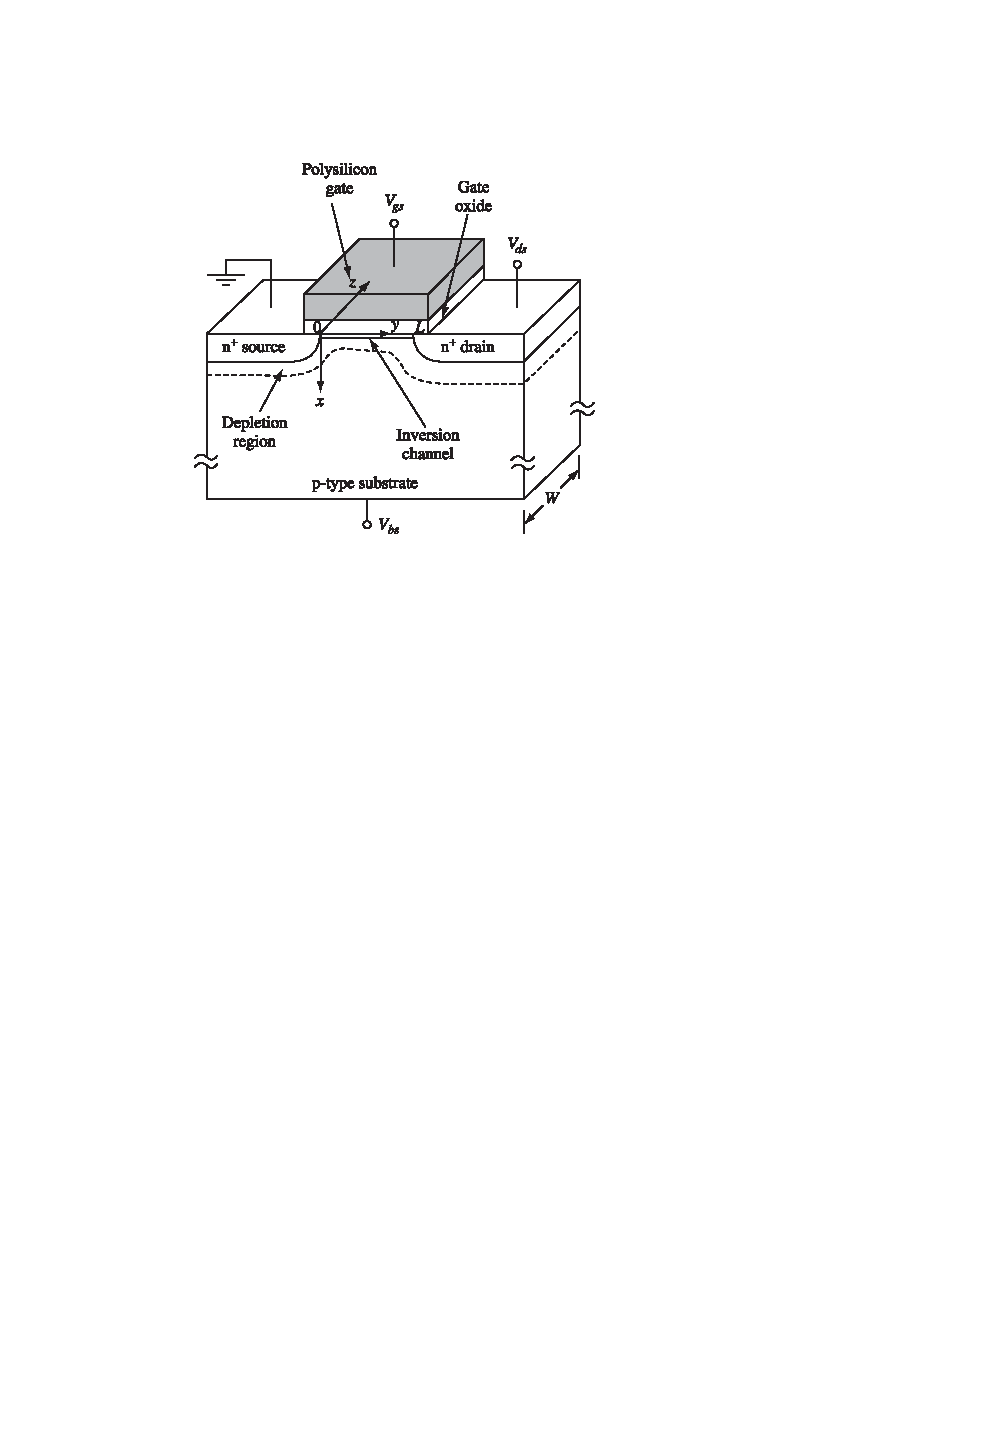
\includegraphics[width=0.5\textwidth]{mosfet_3d.pdf}
    \caption{MOSFET 结构\cite{Modern-VLSI}}
    \label{fig:mosfet_3d}
\end{figure}

%%%
\section{Long-Channel MOSFET I-V Characteristics}

MOSFET 有线性(linear)、饱和(saturation)和截止(cutoff)三种工作状态。以 n-channel 为例,其三种工作状态如图 \ref{fig:mosfet_state} 所示。

\begin{figure}[!htb]
    \centering
    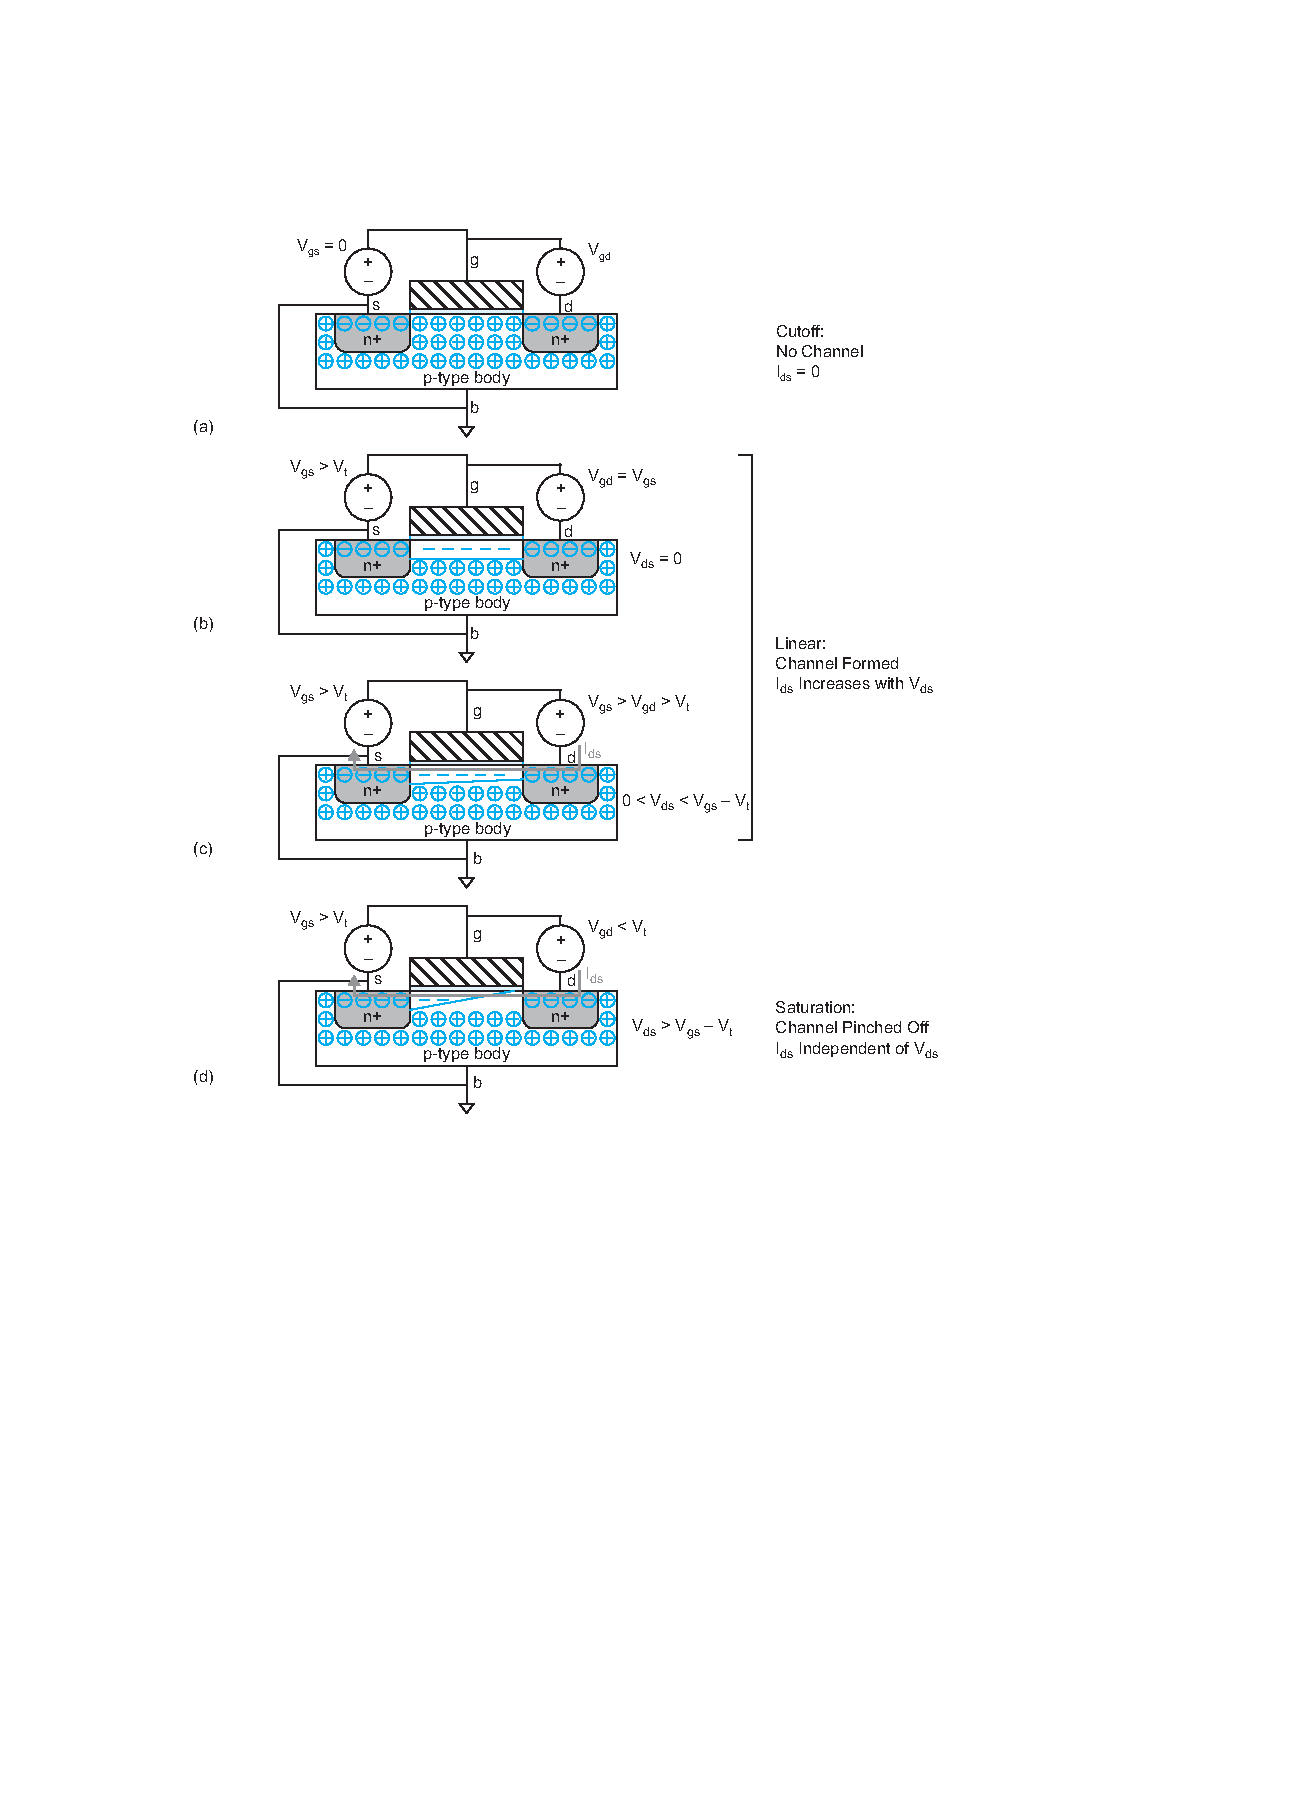
\includegraphics[width=0.7\textwidth]{mosfet_state.pdf}
    \caption{MOSFET 的三种工作状态\cite{CMOS-VLSI}}
    \label{fig:mosfet_state}
\end{figure}

对于 NMOSFET,其 I-V 特性为
\begin{equation}
    I_{\mathrm{D}} = 
    \begin{dcases}  % 自动调整上下两行的高度, dfrac fix
        \begin{aligned}
            & 0 && V_{\mathrm{GS}} < V_{\mathrm{TH}} &&& \text{Cut-off} \\
            & \mu_{\mathrm{n}} C_{\mathrm{ox}} \frac{W}{L} \left[ (V_{\mathrm{GS}} - V_{\mathrm{TH}}) V_{\mathrm{DS}} - \frac{V_{\mathrm{DS}}^2}{2} \right] && V_{\mathrm{GS}} \geqslant V_{\mathrm{TH}}, V_{\mathrm{DS}} \leqslant V_{\mathrm{GS}} - V_{\mathrm{TH}} &&& \text{Linear} \\
            & \frac{1}{2} \mu_{\mathrm{n}} C_{\mathrm{ox}} \frac{W}{L} (V_{\mathrm{GS}} - V_{\mathrm{TH}})^2 && V_{\mathrm{GS}} \geqslant V_{\mathrm{TH}}, V_{\mathrm{DS}} > V_{\mathrm{GS}} - V_{\mathrm{TH}} &&& \text{Saturation}
        \end{aligned}
    \end{dcases}
\end{equation}
对于 PMOSFET,其 I-V 特性为
\begin{equation}
    I_{\mathrm{D}} = 
    \begin{dcases}  % 自动调整上下两行的高度, dfrac fix
        \begin{aligned}
            & 0 && V_{\mathrm{GS}} > V_{\mathrm{TH}} &&& \text{Cut-off} \\
            & \mu_{\mathrm{p}} C_{\mathrm{ox}} \frac{W}{L} \left[ (V_{\mathrm{GS}} - V_{\mathrm{TH}}) V_{\mathrm{DS}} - \frac{V_{\mathrm{DS}}^2}{2} \right] && V_{\mathrm{GS}} \leqslant V_{\mathrm{TH}}, V_{\mathrm{DS}} \geqslant V_{\mathrm{GS}} - V_{\mathrm{TH}} &&& \text{Linear} \\
            & \frac{1}{2} \mu_{\mathrm{p}} C_{\mathrm{ox}} \frac{W}{L} (V_{\mathrm{GS}} - V_{\mathrm{TH}})^2 && V_{\mathrm{GS}} \leqslant V_{\mathrm{TH}}, V_{\mathrm{DS}} < V_{\mathrm{GS}} - V_{\mathrm{TH}} &&& \text{Saturation}
        \end{aligned}
    \end{dcases}
\end{equation}

%%%
\section{Nonideal I-V Effects}

%%%%
\subsection{Mobility Degradation and Velocity Saturation}

沟道较短的晶体管,也称为短沟器件的行为与长沟器件有所不同,它们不再发生夹断饱和(Pinch-Off Saturation),取而代之的是\textbf{速度饱和(Velocity Saturation)}。

若同时考虑\textbf{速度饱和(Velocity Saturation)}效应,对于 NMOSFET,其 I-V 特性为
\begin{equation}
    I_{\mathrm{D}} = 
    \begin{dcases}  % 自动调整上下两行的高度, dfrac fix
        \begin{aligned}
            & 0 && \text{Cut-off} \\
            & \mu_{\mathrm{n}} C_{\mathrm{ox}} \frac{W}{L} \left[ (V_{\mathrm{GS}} - V_{\mathrm{TH}}) V_{\mathrm{DS}} - \frac{V_{\mathrm{DS}}^2}{2} \right] && \text{Linear} \\
            & \frac{1}{2} \mu_{\mathrm{n}} C_{\mathrm{ox}} \frac{W}{L} (V_{\mathrm{GS}} - V_{\mathrm{TH}})^2 && \text{Saturation} \\
            & \mu_{\mathrm{n}} C_{\mathrm{ox}} \frac{W}{L} \left[ (V_{\mathrm{GS}} - V_{\mathrm{TH}}) V_{\mathrm{DSAT}} - \frac{V_{\mathrm{DSAT}}^2}{2} \right] && \text{Velocity Saturation}
        \end{aligned}
    \end{dcases}
\end{equation}
各个状态的电压关系为
\begin{equation}
    \begin{aligned}
        & \text{Cut-off:} && V_{\mathrm{GS}} < V_{\mathrm{TH}} \\
        & \text{Linear:} && V_{\mathrm{GS}} \geqslant V_{\mathrm{TH}}, \min \left(V_{\mathrm{GS}} - V_{\mathrm{TH}}, V_{\mathrm{DS}}, V_{\mathrm{DSAT}}\right) = V_{\mathrm{DS}} \\
        & \text{Saturation:} && V_{\mathrm{GS}} \geqslant V_{\mathrm{TH}}, \min \left(V_{\mathrm{GS}} - V_{\mathrm{TH}}, V_{\mathrm{DS}}, V_{\mathrm{DSAT}}\right) = V_{\mathrm{GS}} - V_{\mathrm{TH}} \\
        & \text{Velocity Saturation:} && V_{\mathrm{GS}} \geqslant V_{\mathrm{TH}}, \min \left(V_{\mathrm{GS}} - V_{\mathrm{TH}}, V_{\mathrm{DS}}, V_{\mathrm{DSAT}}\right) = V_{\mathrm{DSAT}}
    \end{aligned}
\end{equation}
而对于 PMOSFET,其 I-V 特性公式与 NMOSFET 相同,但得到的 $I_{\mathrm{D}}$ 为负值。
\begin{equation}
    I_{\mathrm{D}} = 
    \begin{dcases}  % 自动调整上下两行的高度, dfrac fix
        \begin{aligned}
            & 0 && \text{Cut-off} \\
            & -\mu_{\mathrm{p}} C_{\mathrm{ox}} \frac{W}{L} \left[ (V_{\mathrm{GS}} - V_{\mathrm{TH}}) V_{\mathrm{DS}} - \frac{V_{\mathrm{DS}}^2}{2} \right] && \text{Linear} \\
            & -\frac{1}{2} \mu_{\mathrm{p}} C_{\mathrm{ox}} \frac{W}{L} (V_{\mathrm{GS}} - V_{\mathrm{TH}})^2 && \text{Saturation} \\
            & -\mu_{\mathrm{p}} C_{\mathrm{ox}} \frac{W}{L} \left[ (V_{\mathrm{GS}} - V_{\mathrm{TH}}) V_{\mathrm{DSAT}} - \frac{V_{\mathrm{DSAT}}^2}{2} \right] && \text{Velocity Saturation}
        \end{aligned}
    \end{dcases}
\end{equation}
各个状态的电压关系为
\begin{equation}
    \begin{aligned}
        & \text{Cut-off:} && V_{\mathrm{GS}} > V_{\mathrm{TH}} \\
        & \text{Linear:} && V_{\mathrm{GS}} \leqslant V_{\mathrm{TH}}, \max \left(V_{\mathrm{GS}} - V_{\mathrm{TH}}, V_{\mathrm{DS}}, V_{\mathrm{DSAT}}\right) = V_{\mathrm{DS}} \\
        & \text{Saturation:} && V_{\mathrm{GS}} \leqslant V_{\mathrm{TH}}, \max \left(V_{\mathrm{GS}} - V_{\mathrm{TH}}, V_{\mathrm{DS}}, V_{\mathrm{DSAT}}\right) = V_{\mathrm{GS}} - V_{\mathrm{TH}} \\
        & \text{Velocity Saturation:} && V_{\mathrm{GS}} \leqslant V_{\mathrm{TH}}, \max \left(V_{\mathrm{GS}} - V_{\mathrm{TH}}, V_{\mathrm{DS}}, V_{\mathrm{DSAT}}\right) = V_{\mathrm{DSAT}}
    \end{aligned}
\end{equation}

%%%%
\subsection{Channel Length Modulation}
沟道长度调制(Channel Length Modulation)是指沟道长度的变化会导致沟道电阻的变化,从而影响沟道电流。当栅和漏之间的电压差增大时,实际的反型沟道长度逐渐减小。
假设$\Delta L / L$与$V_{\mathrm{DS}}$为线性关系,满足
\begin{equation}
    \frac{\Delta L}{L} = \lambda V_{\mathrm{DS}}
\end{equation}
其中 $\lambda$ 即为沟道长度调制系数。在饱和区,电流值需要乘上修正系数 $\left(1 + \lambda V_{\mathrm{DS}}\right)$,即
\begin{equation}
    I_{\mathrm{D}} = \frac{1}{2} \mu_{\mathrm{n}} C_{\mathrm{ox}} \frac{W}{L} \left( V_{\mathrm{GS}} - V_{\mathrm{TH}} \right)^2 \eqnmark[RoyalPurple]{lb}{\left( 1 + \lambda V_{\mathrm{DS}} \right)}
\end{equation}
需要注意,沟道长度调制仅在饱和区生效,只有在饱和区才会出现沟道长度的变化$\Delta L$。

\begin{figure}
    \centering
    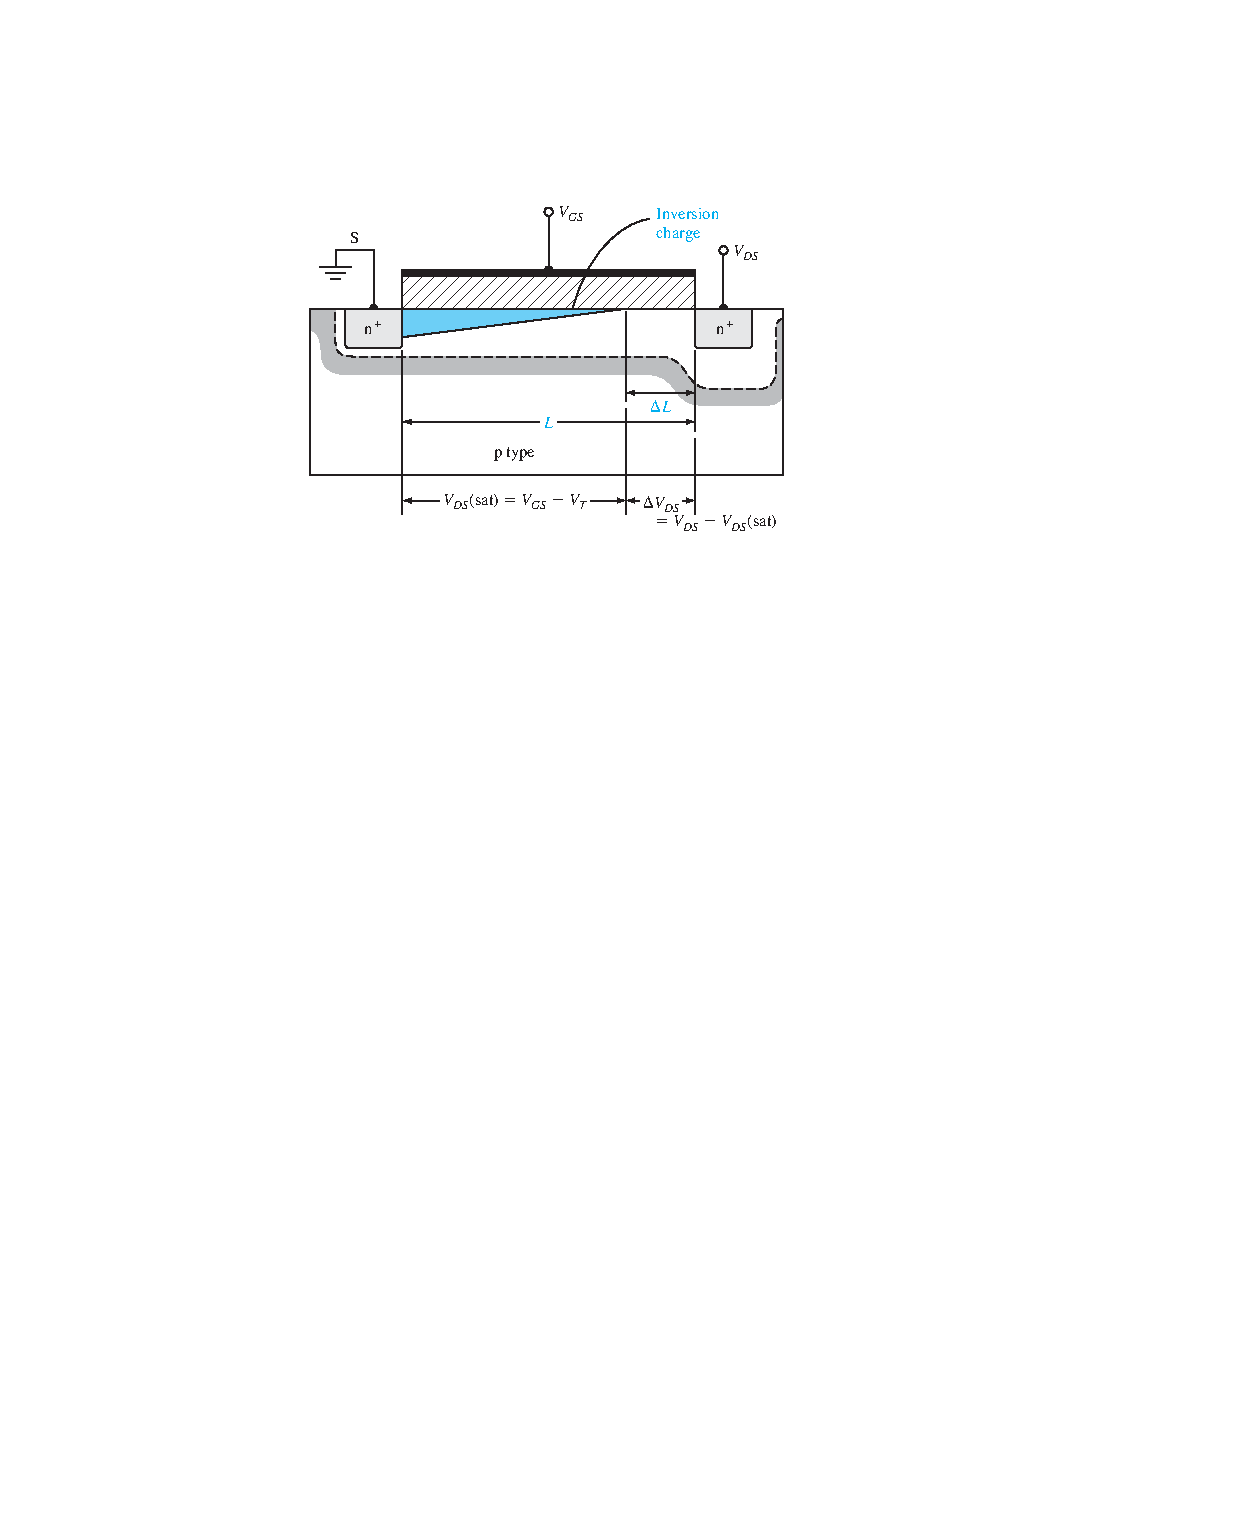
\includegraphics[width=0.7\textwidth]{channel_length_modulation.pdf}
    \caption{沟道长度调制\cite{NeamenSemiconductor}}
    \label{fig:channel_length_modulation}
\end{figure}

%%%%
\subsection{Subthreshold Conduction}

%%%
\subsection{Threshold Voltage Effects}
\subsubsection{Body Effect}

\subsubsection{Drain-Induced Barrier Lowering}

\subsubsection{Short Channel Effect}

%%%
\section{MOSFET I-V Characteristics Summary}

为了简化公式,引入工艺因子(Gain Factor)和工艺跨导(Transconductance)的概念。\\
工艺因子 $k$ 为
\begin{equation}
    \begin{aligned}
        k_{\mathrm{n}} &= \mu_{\mathrm{n}} C_{\mathrm{ox}} \frac{W}{L} \\
        k_{\mathrm{p}} &= -\mu_{\mathrm{p}} C_{\mathrm{ox}} \frac{W}{L}
    \end{aligned}
\end{equation}
工艺跨导 $k'$ 为
\begin{equation}
    \begin{aligned}
        k'_{\mathrm{n}} &= \mu_{\mathrm{n}} C_{\mathrm{ox}} \\
        k'_{\mathrm{p}} &= -\mu_{\mathrm{p}} C_{\mathrm{ox}}
    \end{aligned}
\end{equation}

这样,NMOSFET 的 I-V 特性为(非截止区)
\begin{equation}
    I_{\mathrm{D}} = k_{\mathrm{n}} \left[ (V_{\mathrm{GS}} - V_{\mathrm{TH}}) V_{\mathrm{min}} - \frac{V_{\mathrm{min}}^2}{2} \right] \left(1 + \lambda V_{\mathrm{DS}}\right)
\end{equation}
其中 $V_{\mathrm{min}} = \min \left(V_{\mathrm{GS}} - V_{\mathrm{TH}}, V_{\mathrm{DS}}, V_{\mathrm{DSAT}}\right)$。\\
PMOSFET 的 I-V 特性为
\begin{equation}
    I_{\mathrm{D}} = k_{\mathrm{p}} \left[ (V_{\mathrm{GS}} - V_{\mathrm{TH}}) V_{\mathrm{max}} - \frac{V_{\mathrm{max}}^2}{2} \right] \left(1 + \lambda V_{\mathrm{DS}}\right)
\end{equation}
其中 $V_{\mathrm{max}} = \max \left(V_{\mathrm{GS}} - V_{\mathrm{TH}}, V_{\mathrm{DS}}, V_{\mathrm{DSAT}}\right)$。

\begin{figure}[!hbt]
    \centering
    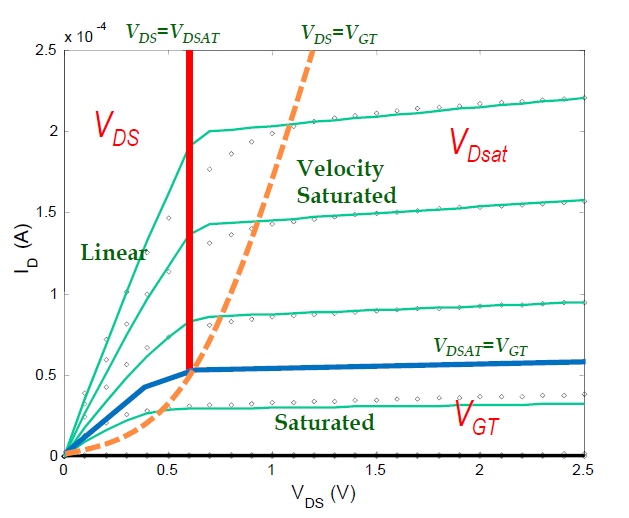
\includegraphics[width=0.5\textwidth]{nmos_iv_regions.png}
    \caption{NMOSFET 的 工作状态}
    \label{fig:nmos_iv_regions}
\end{figure}

%%%
\section{MOSFET C-V Characteristics}

MOSFET 的电容可以概括为栅、漏、源、体四个 terminal 之间的电容,如图 \ref{fig:mosfet_capacitance} 所示。

\begin{figure}[!htb]
    \centering
    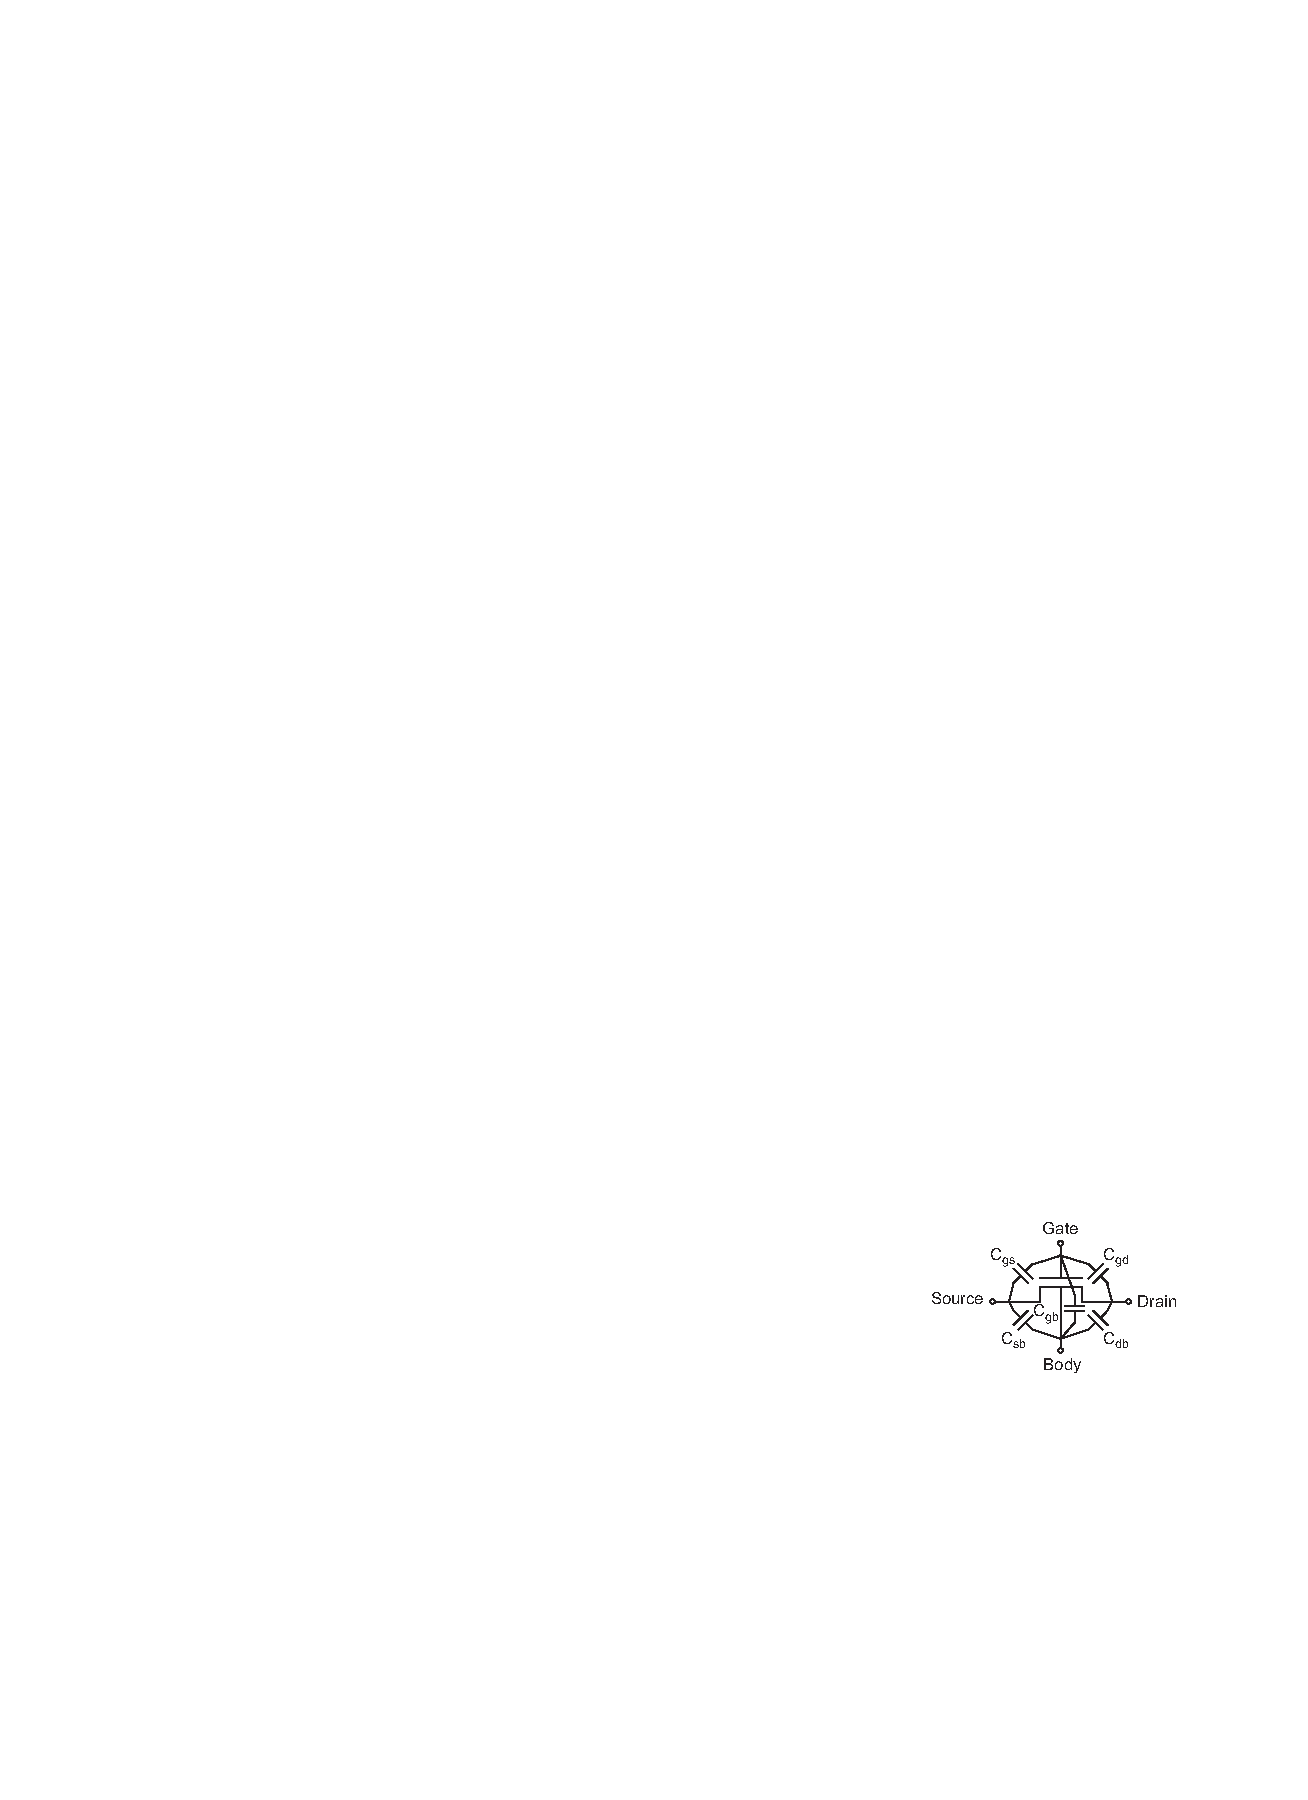
\includegraphics[width=0.5\textwidth]{MOS_Capacitance.pdf}
    \caption{MOSFET 的电容\cite{CMOS-VLSI}}
    \label{fig:mosfet_capacitance}
\end{figure}

电容的来源可以分为以下三部分:
\begin{itemize}
    \item 结构电容(MOS structure capacitances):结构电容是由于 MOS 结构的特性而产生的电容。结构电容的大小与 MOS 结构的面积、厚度、介电常数有关。
    \begin{itemize}
        \item 覆盖电容(Overlap Capacitance):$C_{\mathrm{overlap}} = C_{\mathrm{GSO}} + C_{\mathrm{GDO}}$。覆盖电容是由源和漏在氧化层下延展的横向扩散所引起的栅和源漏间的寄生电容。
    \end{itemize}
    \item 栅至沟道的电容(Gate-to-channel Capacitance):$C_{\mathrm{GC}} = C_{\mathrm{GCB}} + C_{\mathrm{GCS}} + C_{\mathrm{GCD}}$。沟道电容取决于晶体管的工作区间,产生晶体管工作所需的沟道电荷。
    \begin{itemize}
        \item 栅体沟道电容(Gate-Body Channel Capacitance):$C_{\mathrm{GCB}}$。
        \item 栅源沟道电容(Gate-Source Channel Capacitance):$C_{\mathrm{GCS}}$。
        \item 栅漏沟道电容(Gate-Drain Channel Capacitance):$C_{\mathrm{GCD}}$。
    \end{itemize}
    \item 扩散电容/结电容(Juction/Diffusion Capacitance):$C_{\mathrm{diff}} = C_{\mathrm{Sdiff}} + C_{\mathrm{Ddiff}}$。扩散电容/结电容是扩散区处于反向偏置的源体、漏体间的pn结引起的电容。
    \begin{itemize}
        \item 源扩散电容(Source Diffusion Capacitance):$C_{\mathrm{Sdiff}}$。
        \item 漏扩散电容(Drain Diffusion Capacitance):$C_{\mathrm{Ddiff}}$。
    \end{itemize}
\end{itemize}

这样,栅电容 $C_{\mathrm{GS}}$, $C_{\mathrm{GB}}$, $C_{\mathrm{GD}}$ 分别可以表示为
\begin{equation}
    \begin{aligned}
        C_{\mathrm{GS}} &= C_{\mathrm{GCS}} + C_{\mathrm{GSO}} \\
        C_{\mathrm{GB}} &= C_{\mathrm{GCB}} \\
        C_{\mathrm{GD}} &= C_{\mathrm{GCD}} + C_{\mathrm{GDO}}
    \end{aligned}
\end{equation}
结电容 $C_{\mathrm{SB}}$, $C_{\mathrm{DB}}$ 分别可以表示为
\begin{equation}
    \begin{aligned}
        C_{\mathrm{SB}} &= C_{\mathrm{Sdiff}} \\
        C_{\mathrm{DB}} &= C_{\mathrm{Ddiff}}
    \end{aligned}
\end{equation}

电容相关的符号如表 \ref{tab:mosfet-capacitance-symbols} 所示。
\begin{table}[!htb]
    \centering
    \caption{MOSFET 电容符号表}
    \label{tab:mosfet-capacitance-symbols}
    \begin{NiceTabular}{cccc}
        \Xhline{1pt}
        \textbf{Symbol} & \textbf{Meaning} & \textbf{Unit} & \textbf{Polarity} \\ \hline
        $C_{\mathrm{ox}}$ & 单位面积栅氧电容(Gate Oxide Capacitance per unit area) & $\unit{\farad \per \meter \squared}$ & $+$ \\
        $C_{\mathrm{overlap}}$ & 总覆盖电容(Overlap capacitance) & $\unit{\farad}$ & $+$ \\
        $C_{\mathrm{GSO}}$ & 栅源间覆盖电容(Gate-source overlap capacitance) & $\unit{\farad}$ & $+$ \\
        $C_{\mathrm{GDO}}$ & 栅漏间覆盖电容(Gate-drain overlap capacitance) & $\unit{\farad}$ & $+$ \\
        $C_{\mathrm{o}}$ & 单位晶体管宽度覆盖电容(Overlap capacitance per unit transistor width) & $\unit{\farad \per \meter}$ & $+$ \\
        $x_{\mathrm{d}}$ & 横向扩散距离(Lateral diffusion distance) & $\unit{\meter}$ & $+$ \\
        \Xhline{1pt}
    \end{NiceTabular}
\end{table}


%%%%
\subsection{Gate Capacitance}
栅电容可以进一步分为两部分:覆盖电容$C_{\mathrm{overlap}}$和沟道电容$C_{\mathrm{GC}}$。
\subsubsection{Structure Capacitance — Overlap Capacitance}
当通过扩散形成源区和漏区时,理想中,源和漏的扩散应当恰好终止在栅氧的边界上,但是,实际情况是,源和漏的边界都会往栅氧下延伸$x_{\mathrm{d}}$的距离,这被称为横向扩散,这就导致了栅氧覆盖了一定面积的源区和漏区,从而形成了栅和源漏间的\textbf{覆盖电容(Overlap Capacitance)},如图 \ref{fig:overlap_capacitance} 所示。
\begin{figure}[!htb]
    \centering
    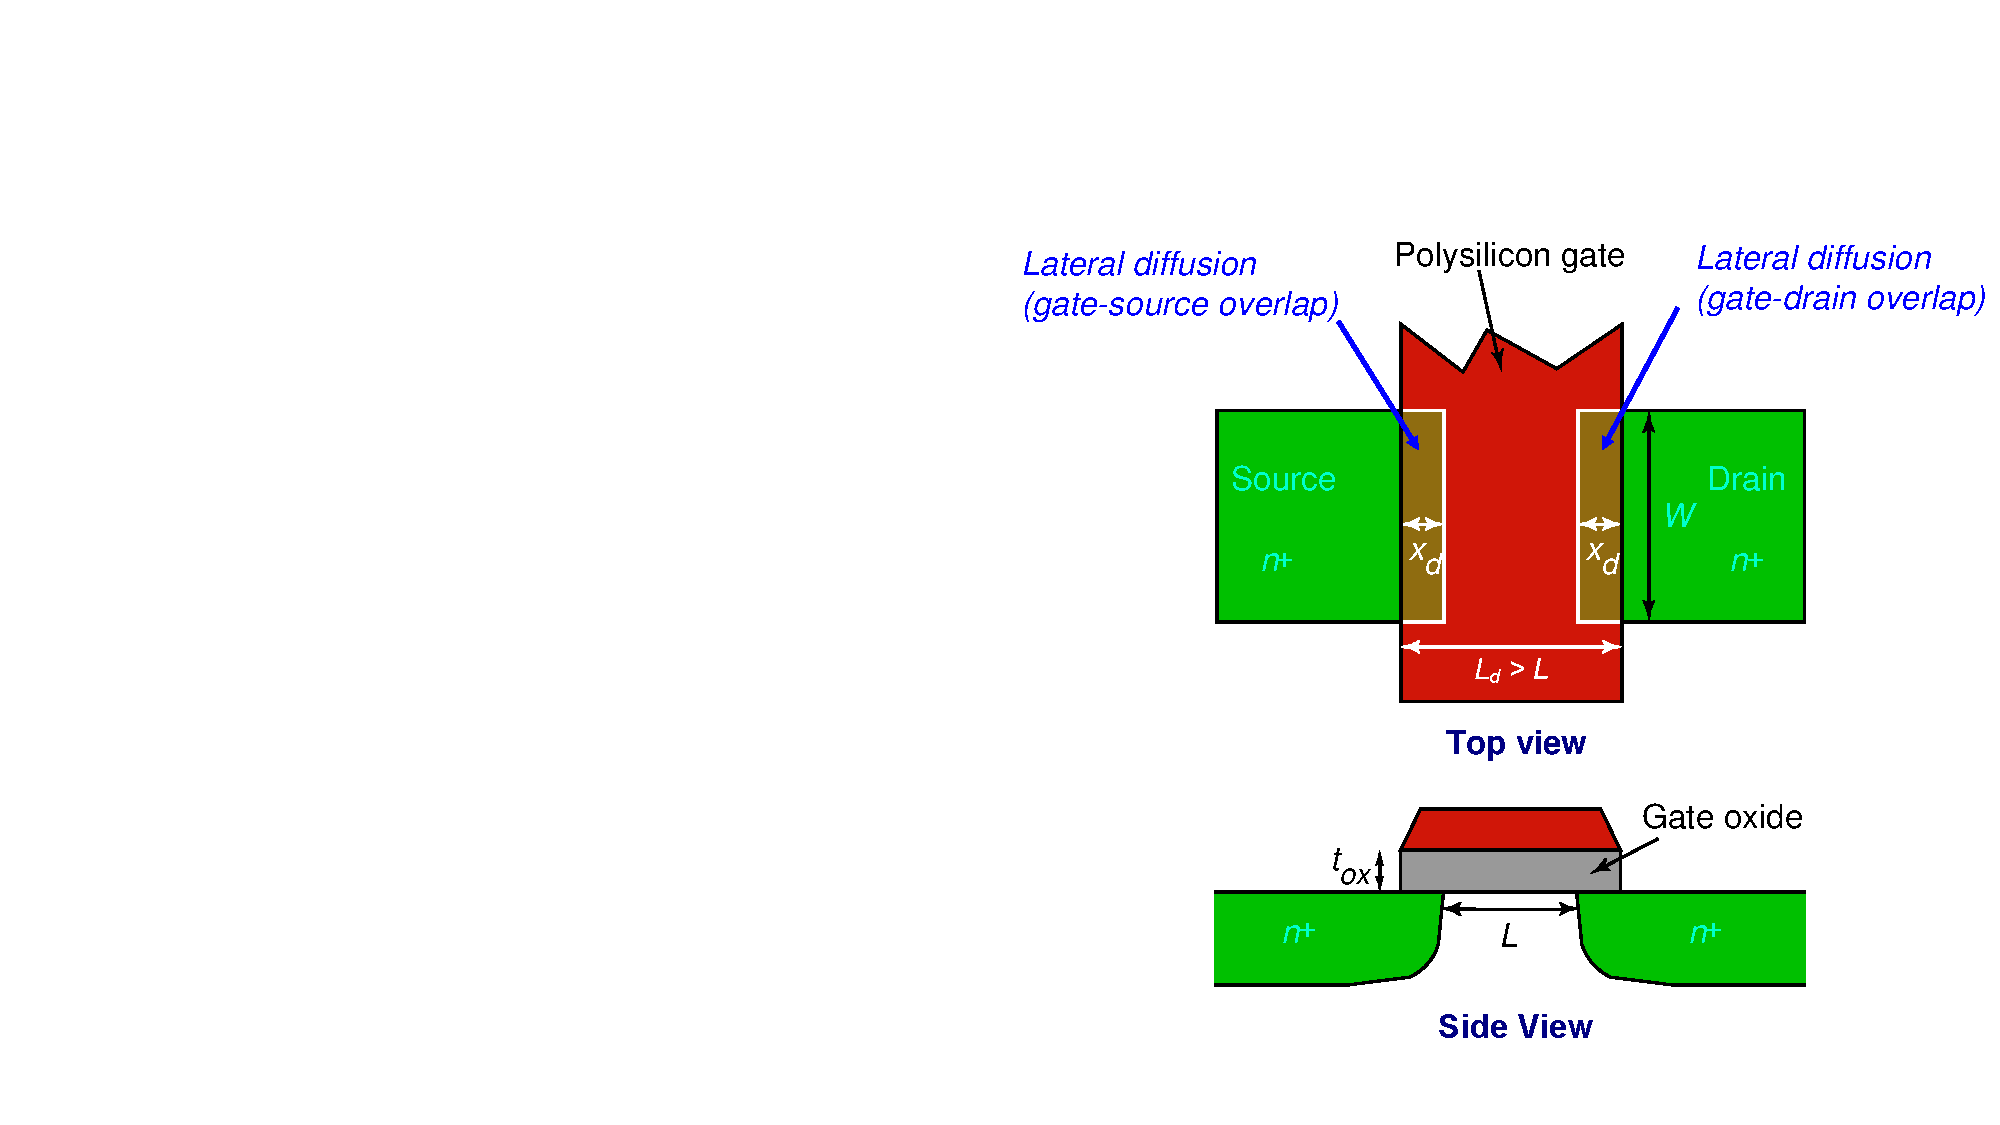
\includegraphics[width=0.5\textwidth]{MOS_overlap.pdf}
    \caption{覆盖电容}
    \label{fig:overlap_capacitance}
\end{figure}

假设两侧的横向扩散距离相同,即$x_{\mathrm{d}} = x_{\mathrm{dS}} = x_{\mathrm{dD}}$,则覆盖电容为
\begin{equation}
    \begin{aligned}
        C_{\mathrm{GSO}} &= C_{\mathrm{GDO}} = C_{\mathrm{ox}} x_{\mathrm{d}} W = C_{\mathrm{o}} W \\
        C_{\mathrm{overlap}} &= C_{\mathrm{GSO}} + C_{\mathrm{GDO}} = 2 C_{\mathrm{ox}} x_{\mathrm{d}} W = 2 C_{\mathrm{o}} W \\
    \end{aligned}
\end{equation}
其中 $C_{\mathrm{ox}}$ = ${\varepsilon_{\mathrm{ox}}}$ / ${t_{\mathrm{ox}}}$。

\subsubsection{Gate-to-Channel Capacitance}
沟道电容的计算可以使用一个简单的线性化模型,如表 \ref{tab:gate2channel-model} 所示。
\begin{table}[h!tb]
    \centering
    \caption{沟道电容模型}
    \label{tab:gate2channel-model}
    \begin{NiceTabular}{c|cccc}
        \Xhline{1pt}
        Operation Region & $C_{\mathrm{GCB}}$ & $C_{\mathrm{GCS}}$ & $C_{\mathrm{GCD}}$ & $C_{\mathrm{GC}} = C_{\mathrm{GCB}} + C_{\mathrm{GCS}} + C_{\mathrm{GCD}}$ \\ \hline
        cut-off & $C_{\mathrm{ox}}WL$ & 0 & 0 & $C_{\mathrm{ox}}WL$ \\ \hline
        linear & 0 & $C_{\mathrm{ox}}WL/2$ & $C_{\mathrm{ox}}WL/2$ & $C_{\mathrm{ox}}WL$ \\ \hline
        saturation & 0 & $2/3C_{\mathrm{ox}}WL$ & 0 & $2/3C_{\mathrm{ox}}WL$ \\
        \Xhline{1pt}
    \end{NiceTabular}
\end{table}

三种工作状态下的沟道电容如图 \ref{fig:gate2channel-capacitance} 所示。
\begin{figure}[hbp]
    \centering
    \begin{subfigure}[b]{0.4\textwidth}
        \centering
        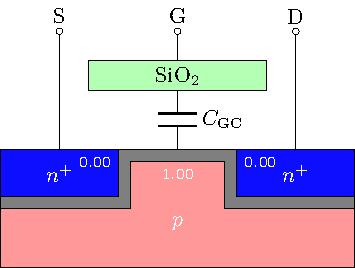
\includegraphics[width=6cm]{C_GC_cutoff.pdf}
        \caption{截止区}
    \end{subfigure}
    \begin{subfigure}[b]{0.4\linewidth}
        \centering
        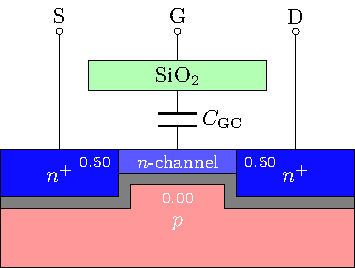
\includegraphics[width=6cm]{C_GC_linear.pdf}
        \caption{线性区}
    \end{subfigure}
    \begin{subfigure}[b]{\linewidth}
        \centering
        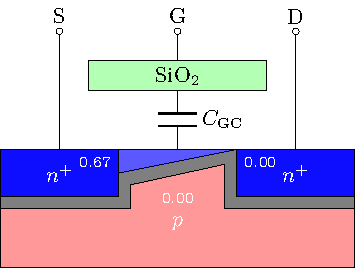
\includegraphics[width=6cm]{C_GC_saturation.pdf}
        \caption{饱和区}
    \end{subfigure}
    \caption{三种工作状态下的沟道电容\cite{DigitalIC_lyx}}
    \label{fig:gate2channel-capacitance}
\end{figure}
